% 第四章 系统总体设计
% 修改说明：本章根据原 chapter4.tex 进行压缩与重组，重点保留总体设计内容，删除过细的实现算法、重复流程描述和过长的 Redis key 细节。

\chapter{系统架构及数据库设计}

\section{系统总体架构设计}
\label{sec:overall-architecture-design}

\subsection{系统总体架构}
\label{subsec:system-overall-architecture}

系统总体架构如图~\ref{fig:system-architecture} 所示。

\begin{figure}[H]
    \centering
    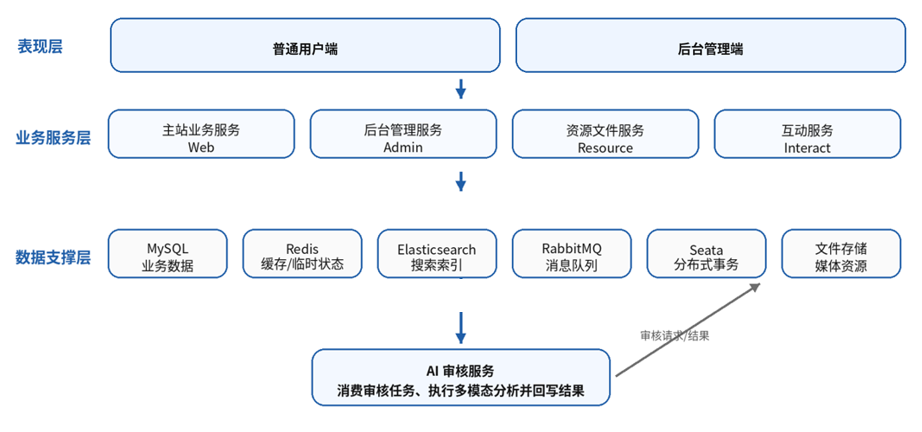
\includegraphics[width=0.95\textwidth]{images/system_architecture.png}
    \caption{系统总体架构图}
    \label{fig:system-architecture}
\end{figure}

图~\ref{fig:system-architecture} 中的架构是围绕用户访问、业务处理、资源处理、AI审核和数据支撑等部分进行分层设计。各层之间通过网关转发、服务调用、消息队列和数据存储组件进行协作，从而支撑视频投稿、转码、审核、发布、播放和互动等核心业务流程。

\noindent\textbf{（1）表现层。}
表现层可分成普通用户端和后台管理端。普通用户端提供视频浏览、关键词搜索、视频播放、投稿上传、评论弹幕、点赞收藏等功能入口；后台管理端提供分类管理、视频审核、AI 审核结果查看、内容管理等功能入口。表现层只需将请求通过网关转发给后端服务处理复杂业务逻辑。

\noindent\textbf{（2）业务服务层。}
业务服务层是系统核心业务处理部分，业务服务分成了主站业务服务、后台管理服务、资源文件服务和互动服务。主站业务服务负责用户信息、首页数据、视频信息、投稿信息、搜索编排和 AI 审核任务创建等业务；后台管理服务负责管理员登录、分类维护、视频审核和审核结果查看；资源文件服务负责封面图片上传、视频分片上传、分片合并、视频转码和 HLS 播放资源输出文件处理等；互动服务负责评论、弹幕、点赞、收藏和投币等高频互动行为。服务的拆分可以避免所有业务都集中于单个服务，也可以降低模块之间的耦合度。

\noindent\textbf{（3）AI 能力层。}
AI 能力层负责处理AI视频的审核。在视频完成转码后，主站业务服务会创建审核任务，将任务交给消息队列向 AI 审核服务发送审核请求。AI 审核服务消费任务后会对视频内容进行分析，并将审核结果返回给后端业务服务。AI 服务不会被某个服务直接内部调用，而是通过异步方式与后端服务通信。并且服务返回的结果是为管理员人工审核提供辅助判断依据，由后台审核流程控制。

\noindent\textbf{（4）数据支撑层。}
数据支撑层为系统运行提供基础数据能力，主要包括 MySQL、Redis、Elasticsearch、RabbitMQ、Seata 和本地文件目录等。MySQL 用于存储核心业务数据；Redis 用于保存临时状态、缓存数据和轻量队列数据；Elasticsearch 则用于建立视频搜索索引，提高关键词检索能力；RabbitMQ支撑AI审核任务的异步投递和结果回传；Seata 支撑跨服务写操作的数据一致性；本地文件目录用于保存封面、上传分片、转码视频、HLS 切片和 AI 审核截图等媒体资源。

\section{微服务模块划分}
\label{sec:microservice-module-design}

\subsection{系统服务模块说明}
\label{subsec:service-module-description}

\begin{table}[htbp]
    \centering
    \caption{系统服务模块及职责}
    \label{tab:service-modules}
    \begin{tabular}{p{0.37\textwidth}p{0.14\textwidth}p{0.39\textwidth}}
    \hline
    \textbf{模块名称} & \textbf{网关前缀} & \textbf{主要职责} \\
    \hline
    \texttt{streama-cloud-gateway} & -- & API 统一入口、路由转发、内部接口隔离、管理端过滤 \\
    \texttt{streama-cloud-web} & \texttt{/web} & 用户、首页、视频信息、投稿、搜索和 AI 审核任务编排 \\
    \texttt{streama-cloud-admin} & \texttt{/admin} & 管理端登录、分类管理、视频审核、审核结果查询 \\
    \texttt{streama-cloud-resource} & \texttt{/file} & 图片上传、视频分片上传、视频转码和 HLS 资源输出 \\
    \texttt{streama-cloud-interact} & \texttt{/interact} & 评论、弹幕、点赞、收藏等互动行为处理 \\
    \texttt{streama-cloud-common} & -- & Redis、搜索、异常处理、公共组件和工具类 \\
    \texttt{streama-cloud-base} & -- & 常量、枚举、基础实体和公共 DTO \\
    \texttt{ai-service} & -- & 消费审核任务，执行多模态审核返回审核结果 \\
    \hline
    \end{tabular}
\end{table}

系统服务模块及其职责如表~\ref{tab:service-modules} 所示。

主站服务应对于 web 模块，处理业务核心的模块，但不是所有功能的承载点。每个服务分别为其解耦。文件处理可以集中交给资源服务模块 resource 管理；用户与用户之间的互动如评论、弹幕等可拆分给互动服务模块 interact 。后台服务模块 admin 的解耦可以使管理员接口和普通用户接口更容易区分。common 模块和 base 模块则提供了跨服务的公共组件和基础数据结构，避免重复开发。AI 服务模块 则独立部署，专注于 AI 审核任务的处理。

\subsection{服务协作关系}
\label{subsec:service-call-relation}

各服务之间围绕着具体业务场景协作。当用户提交投稿信息时，主站服务负责保存投稿主数据和分 P 文件数据，主数据为视频的标题，简介等信息；P文件数据代表这这个视频可能包含多个视频文件，以待转码文件的形式加入队列；资源服务消费队列后完成视频转码，并回写转码结果；当全部分 P 转码完成后，主站服务会创建 AI 审核任务并发送消息；AI 服务审核完成后回传结果；管理员最终在后台完成复核与发布操作。

\begin{table}[htbp]
    \centering
    \caption{系统主要服务调用关系}
    \label{tab:service-call-relations}
    \begin{tabular}{p{0.18\textwidth}p{0.24\textwidth}p{0.18\textwidth}p{0.30\textwidth}}
    \hline
    \textbf{调用方} & \textbf{被调用方} & \textbf{调用方式} & \textbf{主要用途} \\
    \hline
    网关服务 & 主站/后台/资源/互动服务 & 路由转发 & 将外部请求转发到对应服务 \\
    主站服务 & 后台服务 & 同步调用 & 获取分类树和分类列表 \\
    主站服务 & 互动服务 & 同步调用 & 查询用户互动状态，联动处理互动数据 \\
    资源服务 & 主站服务 & 内部接口 & 回写视频转码结果和文件信息 \\
    主站服务 & AI 审核服务 & 消息队列 & 发送审核请求并接收审核结果 \\
    后台服务 & 主站服务 & 内部接口 & 查询待审核视频并提交人工审核结果 \\
    \hline
    \end{tabular}
\end{table}

由表~\ref{tab:service-modules}对服务与服务之间调用关系和用途进行简单的说明，这种调用关系将同步请求和异步任务进行了区分。对查询分类、查询互动状态等轻量业务，可以采用同步调用；对视频转码、AI 审核等耗时任务，则使用队列异步处理，避免用户请求长时间阻塞。

\section{数据库设计}
\label{sec:database-overall-design}

\subsection{核心数据表与投稿发布数据设计}

本系统核心数据围绕“用户—视频—互动”三类对象展开，整体结构如图~\ref{fig:core-database-er}所示。
其核心业务实体包括分类、用户、关注关系、视频主数据与文件、评论、弹幕及用户行为等，视频信息共同构成“投稿态”与“正式发布态”双态并存的数据架构。

\begin{figure}[htbp]
    \centering
    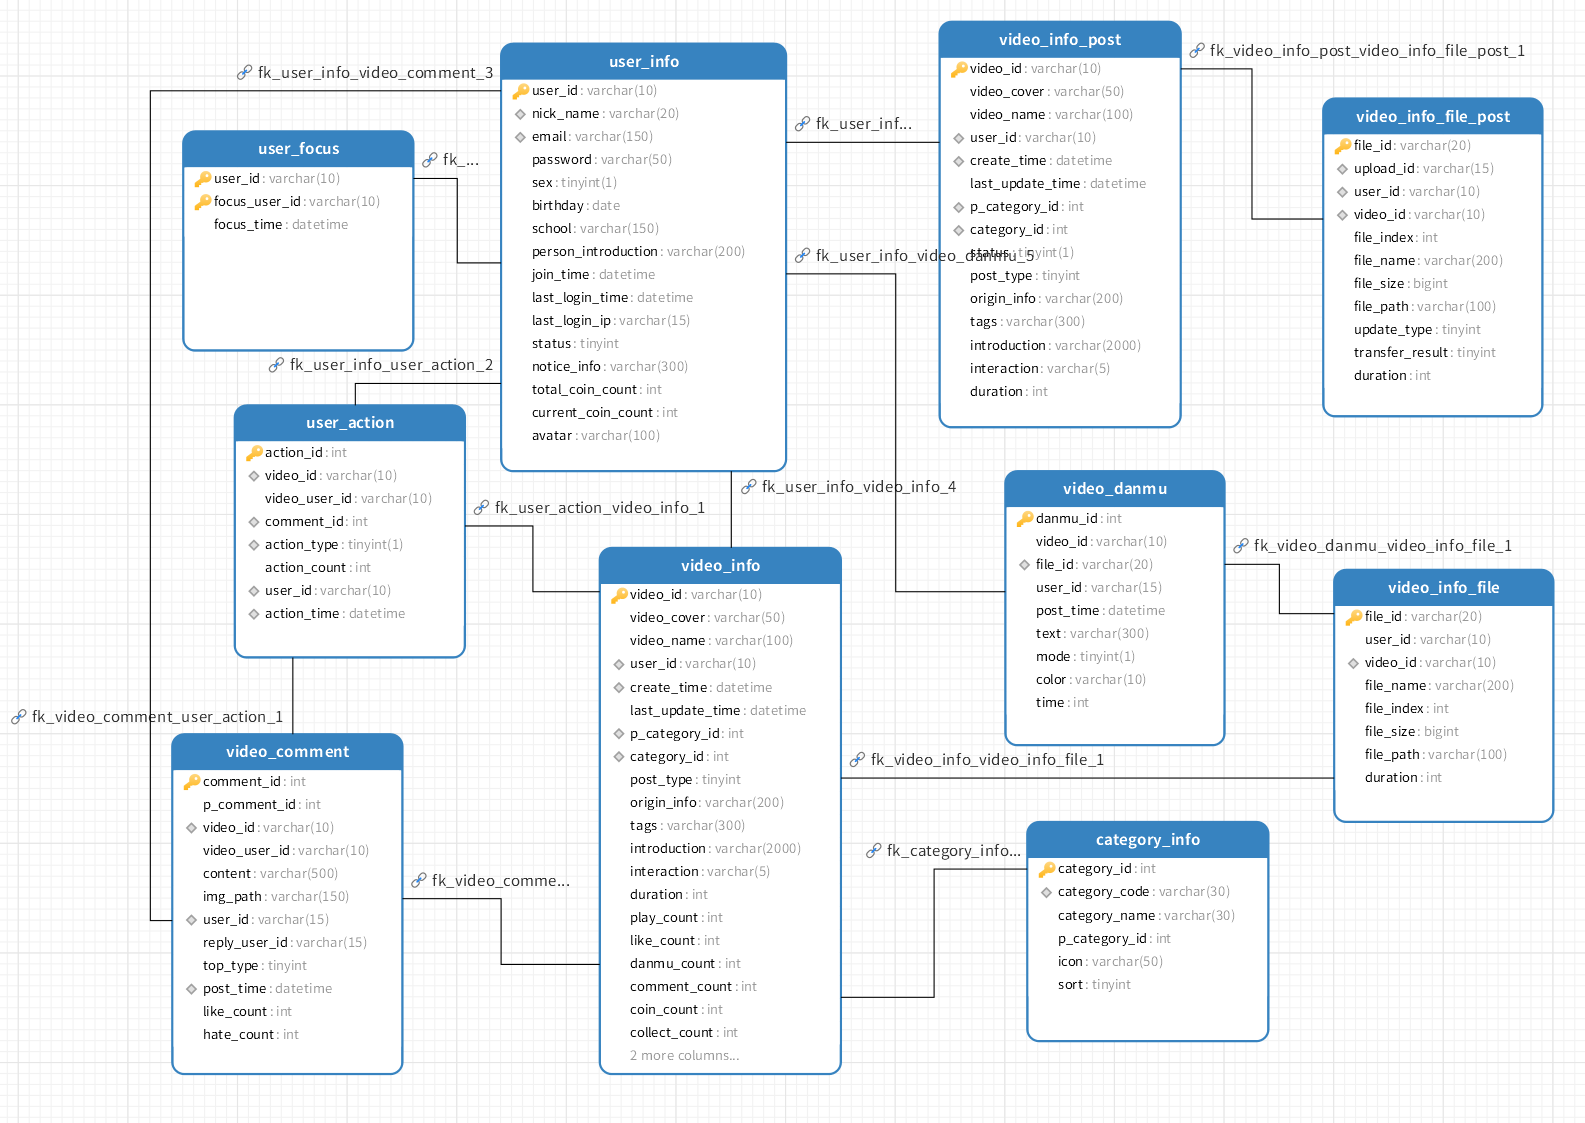
\includegraphics[width=0.98\textwidth]{images/core_database_er.png}
    \caption{核心业务数据库 ER 图}
    \label{fig:core-database-er}
\end{figure}

各表的核心字段与职责如下：

（1）\texttt{category\_info}：视频分类表。核心字段\texttt{category\_id}、\texttt{p\_category\_id} 和 \texttt{sort} 支撑一级与二级分类的层级展示、投稿选择及筛选检索。

（2）\texttt{user\_info}：用户基础信息表。融合账号认证（邮箱、密码）与业务数据（硬币余额、状态、个人介绍），是登录、投稿、互动及统计分析的核心基础。

（3）\texttt{user\_focus}：用户关注关系表。通过 \texttt{user\_id} 与 \texttt{focus\_user\_id} 维护关注与粉丝列表，用于主页关注状态展示。

（4）\texttt{video\_info\_post} 与 \texttt{video\_info\_file\_post}：投稿态数据表组，分别存储待审视频的主信息与分P文件及转码状态。其中 \texttt{status}、\texttt{transfer\_result} 等控制字段专用于投稿流程管理，内容不进入公开访问域。

（5）\texttt{video\_info} 与 \texttt{video\_info\_file}：正式发布数据表组，存储审核通过后的视频主信息与播放资源文件。相较投稿表，增加了播放量、互动计数等前台展示所需字段，直接服务于搜索、推荐和在线播放。

（6）\texttt{video\_comment}：视频评论表。利用 \texttt{p\_comment\_id} 实现回复层级，包含点赞点踩计数及置顶标记，支撑评论区完整交互。

（7）\texttt{video\_danmu}：视频弹幕表。记录文本内容、视频内出现时间点及样式信息，服务于弹幕的实时发送与加载。

（8）\texttt{user\_action}：用户行为记录表。通过 \texttt{action\_type} 区分点赞、收藏、投币等操作，为前台展示和后台行为分析提供明细数据。

为保证未审核内容与公开链路的严格隔离，系统在数据层面采用了“先入投稿库，后迁正式库”的分离设计。

创作者提交后，视频主信息和分P文件状态被分别写入 \texttt{video\_info\_post} 与 \texttt{video\_info\_file\_post}，此后经历转码与审核。这期间的投稿态数据仅供内部流程控制，对用户不可见。一旦审核通过，系统自动将核心数据迁移至 \texttt{video\_info} 与 \texttt{video\_info\_file} 等正式发布表，并同步构建前台索引，使视频正式上线。

这一“投稿态—正式态”分离设计，天然将面向流程的写入/更新操作，与面向用户的公开读取操作解耦。它既保障了内容合规审核的数据安全，避免待审或违规内容的外泄，也让前台公开数据保持相对稳定，利于提升检索效率与播放稳定性。同时，各阶段的独立状态控制，增强了业务流程的可管理性和系统的整体可维护性。

\subsection{AI 审核数据设计}
\label{subsec:ai-audit-data-design}

AI 审核数据采用主从结构。\texttt{ai\_audit\_task} 保存视频级审核任务，例如请求编号、视频编号、审核版本、任务状态、AI 建议、风险等级和审核摘要等信息；\texttt{ai\_audit\_task\_item} 保存分 P 级审核结果，例如文件编号、风险分数、风险标签、命中片段和原因说明等信息。

采用主从结构的原因是，一个视频可能包含多个分 P 文件，AI 审核既需要给出整条视频的综合结论，也需要保留每个分 P 的风险细节。如果只保存一个总结果，管理员难以定位风险出现在哪个视频片段；如果只保存明细而没有总结果，审核列表展示又不够直观。

\begin{table}[htbp]
    \centering
    \caption{AI 审核数据设计}
    \label{tab:ai-audit-data-design}
    \begin{tabular}{p{0.25\textwidth}p{0.30\textwidth}p{0.35\textwidth}}
    \hline
    \textbf{数据表} & \textbf{数据粒度} & \textbf{主要字段含义} \\
    \hline
    \texttt{ai\_audit\_task} & 视频级任务 & 请求编号、视频编号、审核版本、任务状态、AI 建议、风险等级、审核摘要 \\
    \texttt{ai\_audit\_task\_item} & 分 P 文件级结果 & 文件编号、风险分数、风险标签、命中片段、关键帧路径、原因说明 \\
    \hline
    \end{tabular}
\end{table}

\section{消息通信与 AI 审核任务设计}
\label{sec:message-async-design}

视频上传、视频转码、AI 审核等操作属于耗时较长的业务流程。如果这些任务在用户请求过程中同步执行，会导致接口响应时间变长，影响用户投稿体验。因此在视频投稿与审核流程中引入异步任务处理机制，将耗时操作从主业务流程中拆分出来，通过消息通信和任务状态管理提高系统的稳定性。

\begin{figure}[htbp]
    \centering
    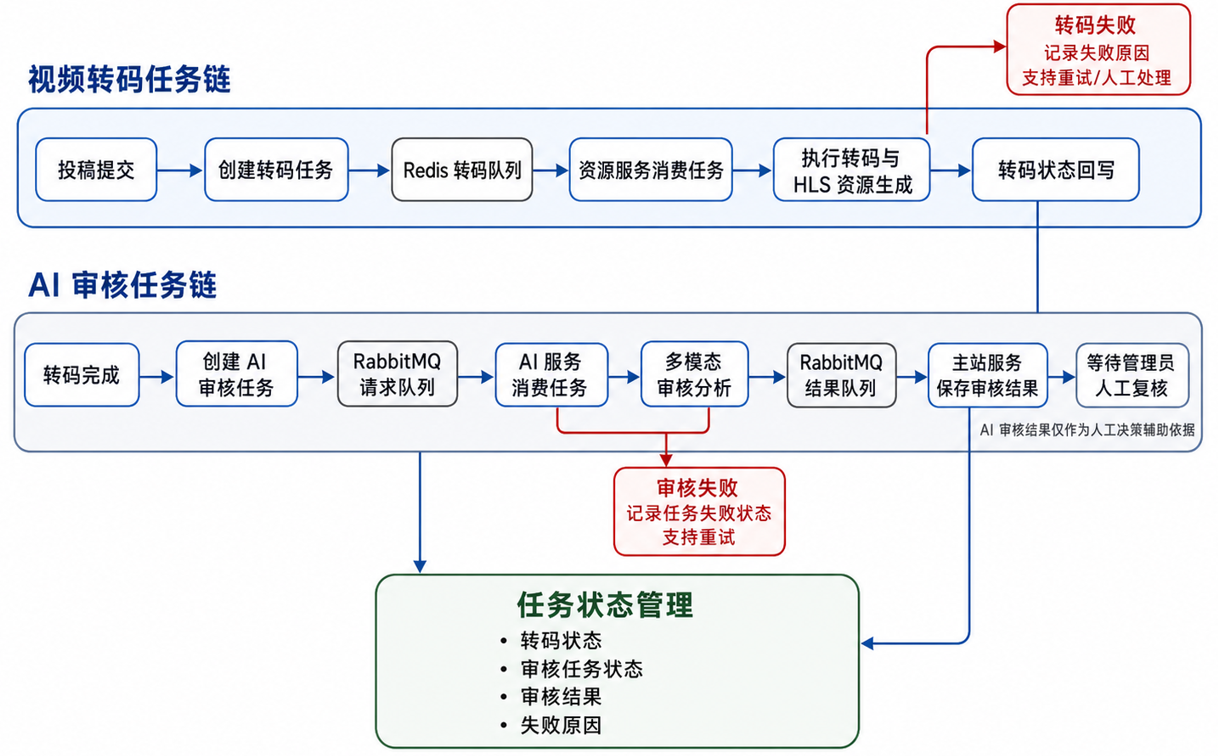
\includegraphics[width=0.95\textwidth]{images/async_task_design.png}
    \caption{异步任务总体流程图}
    \label{fig:async-task-design}
\end{figure}

\subsection{消息通信设计}
\label{subsec:async-task-overall-design}

如图~\ref{fig:async-task-design} 所示，系统的异步任务主要围绕视频投稿后的文件处理流程展开。用户提交视频后，系统先保存投稿态数据以及记录视频文件的基础信息。由于视频文件转码、状态更新和结果回写等操作耗时较长，将相关任务交由后台异步执行。这样可以缩短用户投稿接口的响应时间，同时避免长时间同步处理造成接口阻塞。

消息通信设计的核心目标是实现业务流程解耦。投稿接口只负责完成必要的数据保存和任务创建，后续的文件处理、转码执行和状态更新则由独立的后台任务完成。不同服务之间通过消息或任务记录传递必要的数据，例如视频编号、文件编号、文件路径、任务状态等。处理服务获取任务后，根据任务内容执行对应操作，并在处理完成后更新数据库中的任务状态和业务状态。

任务状态是异步流程控制的重要依据。由于异步任务并不是创建后立即完成，系统需要记录任务在不同阶段的执行情况，例如待处理、处理中、处理成功和处理失败等。通过状态字段，系统可以判断当前任务是否已经被执行、是否执行成功、是否需要重新处理，以及是否可以进入下一业务环节。

\begin{table}[htbp]
    \centering
    \caption{异步任务状态设计}
    \label{tab:async-task-status}
    \begin{tabular}{p{0.20\textwidth}p{0.28\textwidth}p{0.42\textwidth}}
        \hline
        \textbf{状态} & \textbf{含义} & \textbf{处理说明} \\
        \hline
        待处理 & 任务已创建但尚未开始执行 & 等待后台任务消费或定时任务扫描处理 \\
        处理中 & 任务已被获取并正在执行 & 记录任务执行过程，避免重复处理 \\
        处理成功 & 任务正常完成并返回结果 & 更新业务数据，进入下一流程节点 \\
        处理失败 & 任务执行过程出现异常 & 记录失败原因，必要时进行重试或人工处理 \\
        \hline
    \end{tabular}
\end{table}

在异常处理方面，系统需要考虑文件处理失败、转码失败、状态更新失败以及任务长时间未完成等情况。对于可以自动恢复的异常任务，系统可以通过重试机制重新执行；对于多次处理失败或无法自动判断的问题，则需要记录异常原因，并交由管理员进行人工处理。通过任务状态和异常信息的配合，系统能够较好地追踪异步任务的执行过程，避免异常任务影响正常业务流程。

\subsection{AI 审核消息通道设计}
\label{subsec:ai-message-channel-design}

AI 审核任务采用 RabbitMQ 进行消息通信。主站服务作为审核请求生产者，将视频编号、分 P 文件信息、资源路径和任务编号等信息发送到审核请求队列；AI 服务作为消费者，从队列中获取任务并执行审核；审核完成后，AI 服务将结果发送到审核结果队列，主站服务再消费结果并写入数据库。

\begin{table}[htbp]
    \centering
    \caption{AI 审核消息通道设计}
    \label{tab:ai-message-channel}
    \begin{tabular}{p{0.24\textwidth}p{0.36\textwidth}p{0.30\textwidth}}
    \hline
    \textbf{消息组件} & \textbf{名称} & \textbf{作用} \\
    \hline
    Exchange & \texttt{streama.audit.exchange} & AI 审核请求和结果共用交换机 \\
    请求队列 & \texttt{streama.audit.request.queue} & AI 服务消费审核请求 \\
    请求路由键 & \texttt{audit.video.request} & 主站服务发送审核请求时使用 \\
    结果队列 & \texttt{streama.audit.result.queue} & 主站服务消费审核结果 \\
    结果路由键 & \texttt{audit.video.result} & AI 服务发送审核结果时使用 \\
    请求死信队列 & \texttt{streama.audit.request.dlq} & 保存请求处理失败的消息 \\
    结果死信队列 & \texttt{streama.audit.result.dlq} & 保存结果处理失败的消息 \\
    \hline
    \end{tabular}
\end{table}

该消息通道设计包含请求投递、任务消费、结果回传和失败处理。即使 AI 服务暂时不可用，请求消息也可以保留在队列中，等待服务恢复后继续处理。

\section{视频业务流程设计}

\label{sec:video-business-process-design}

视频业务设计流程划分为投稿与资源处理、审核与发布、消费与互动三个阶段。视频业务服务协作流程如图~\ref{fig:video-business-process} 所示。

\begin{figure}[htbp]
    \centering
    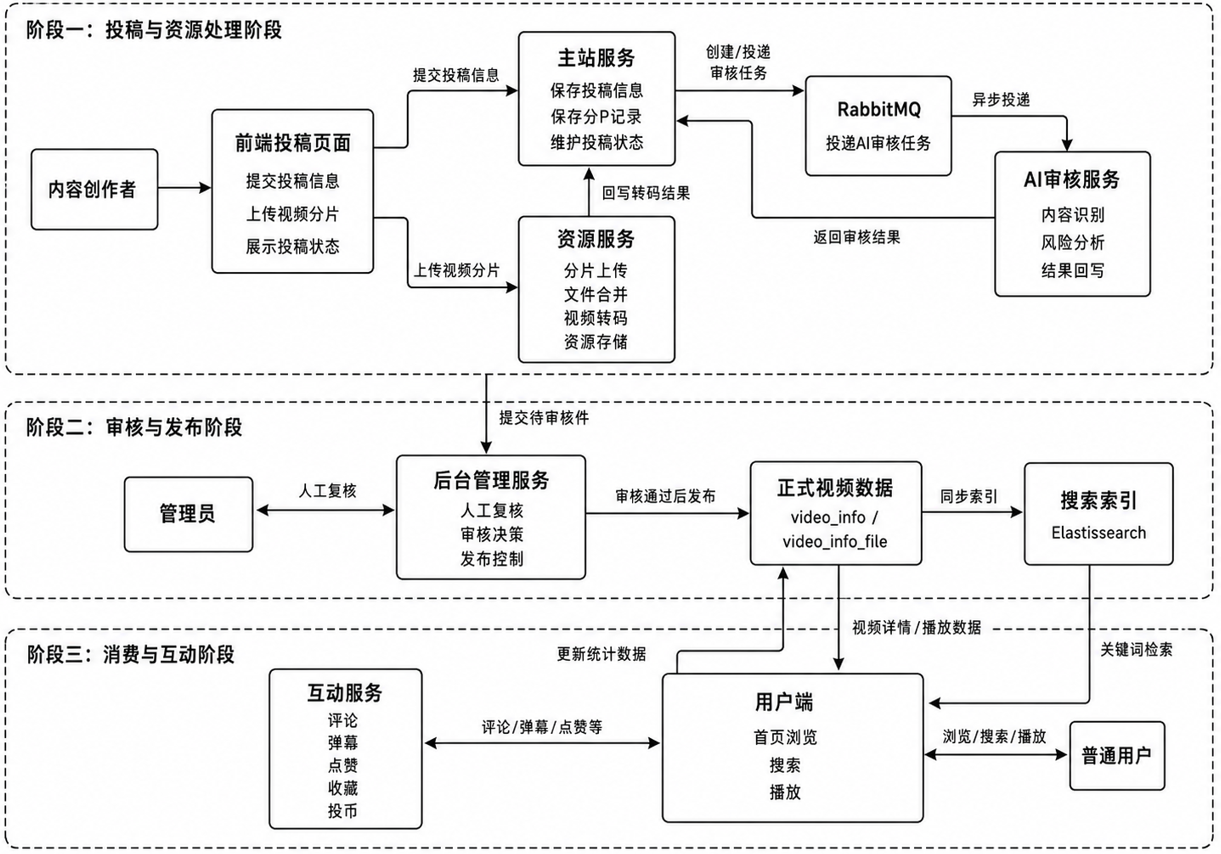
\includegraphics[width=0.95\textwidth]{images/video_business_process.png}
    \caption{视频业务流程设计图}
    \label{fig:video-business-process}
\end{figure}

\subsection{视频投稿与资源处理流程设计}

\label{subsec:video-post-resource-process-design}

视频投稿流程由内容创作者发起，涉及主站服务和资源服务之间的协作。创作者在前端填写视频标题、分类、标签、简介、封面和分 P 文件信息后，系统首先对投稿基础信息进行保存。由于视频文件通常体积较大，资源上传不适合采用普通表单一次性提交，因此系统采用分片上传方式处理视频文件。前端在上传前向资源服务申请上传标识，资源服务根据上传标识保存分片临时文件，并在全部分片上传完成后进行文件合并。

投稿信息与视频资源不是一次性同步完成的。主站服务负责保存视频投稿主数据和分 P 文件记录，资源服务负责处理文件上传、合并、转码和播放资源生成。视频文件转码完成后，资源服务将处理结果回写给主站服务，主站服务再根据各分 P 文件的处理结果判断投稿是否可以进入后续审核阶段。该设计能够避免主站服务直接承担大文件处理任务，也能使视频转码失败时保留明确的处理状态。

该流程中的投稿数据仍处于待处理或待审核状态，不会直接进入前台公开视频列表。

\subsection{视频审核与发布流程设计}

\label{subsec:video-audit-publish-process-design}

视频完成资源处理后，需要进入审核与发布阶段。系统采用 AI 审核辅助和管理员人工复核结合的方式。主站服务在确认视频文件转码完成后，创建 AI 审核任务，并通过消息队列将视频编号、分 P 文件信息和资源路径发送给 AI 审核服务。AI 审核服务消费任务后，对视频内容进行分析，并将风险等级、命中标签、命中片段和审核建议等结果返回给主站服务。

AI 审核结果只作为管理员审核的辅助依据，不直接决定视频最终是否发布。管理员在后台审核页面查看投稿信息、视频内容和 AI 审核结果后，可以选择审核通过或审核不通过。审核通过时，系统将投稿态视频数据转换为正式发布数据，并同步写入正式视频表、正式视频文件表和搜索索引；审核不通过时，系统保留投稿状态和审核结果，避免不符合要求的视频进入用户端展示范围。

这种设计将“自动分析”和“最终决策”分开处理。一方面，AI 审核可以提前发现疑似风险内容，降低管理员审核压力；另一方面，人工复核能够避免完全依赖自动审核带来的误判问题。视频发布结果最终由后台审核流程控制，从而保证内容发布流程的可控性。

\subsection{视频消费与互动流程设计}

\label{subsec:video-consume-interaction-process-design}

视频审核通过并正式发布后，普通用户可以在前台进行浏览、搜索和播放。系统前台展示的数据主要来自正式视频数据，而不是投稿态数据。首页推荐、分类筛选和视频详情页只展示已经通过审核的视频内容，搜索功能则通过 Elasticsearch 索引提高关键词检索效率。这样可以避免待审核、审核失败或转码失败的视频被普通用户访问。

视频播放过程中，用户可以根据视频分 P 信息选择不同片段进行观看。播放资源由资源服务提供，视频基础信息、作者信息和统计信息由主站服务提供。对于评论、弹幕、点赞、收藏、投币等高频互动行为，系统由互动服务单独处理，避免所有操作都集中在主站服务中。互动结果可以再通过统计字段或异步更新方式反映到视频展示数据中。

视频消费流程与投稿审核流程相比，更强调读取效率和用户体验。投稿审核阶段关注的是状态控制和内容安全，视频消费阶段关注的是公开视频的快速查询、稳定播放和互动数据维护。通过将视频投稿、审核发布和用户互动划分为不同流程，系统能够在总体设计上保持较清晰的业务边界。